\chapter{Design and implementation}
\label{chap:design-and-implementation}

\section{Architecture}
\label{sect:architecture}

Since our main stakeholders are students, we decided to base our design decisions on what would attract students to our website. Our colour palette was decided early on, and we focused on a gender neutral, yet colourful and engaging design. Simplicity was something that the entire team wanted; as students, we know how difficult it is to navigate cluttered and confusing websites. Due to this, we were encouraged to ensure that the focus remained on the actual studying and not an immense overload of things to explore. 

---------------------------------------------------------------------------------------------------------------------

The Login and Sign-up pages were created to mirror each other, with a straightforward UI and clear input fields. Any errors are repeated back to the user to ensure a smooth login/sign-up process. 

After the user logs in, they are directed to the main Dashboard page, where there is a ‘mini version’ of each of the features. This way, the user gets an immediate idea of the overview of features, 
without getting overwhelmed. If they wish to ‘expand’ the feature, they can simply click on the relevant icon (e.g. a simplified calendar icon, where if you click it, it brings you to a dedicated calendar page with multiple interactive features you can use). 

Again, with the Group-Study page, we retained a simplified approach. As mentioned before, this is due to the possibility that the user may become distracted if the UI is too cluttered. This idea is reflected in our colour scheme also, with the palette containing subtle and light colours that are easy on the eyes.


\subsection{Database Design Details}

Our system consists of a relational database (Django Models) for structured data and Firebase for media storage. Below is our finalised ER diagram, representing all the Django models used:

\begin{figure}
    \centering
    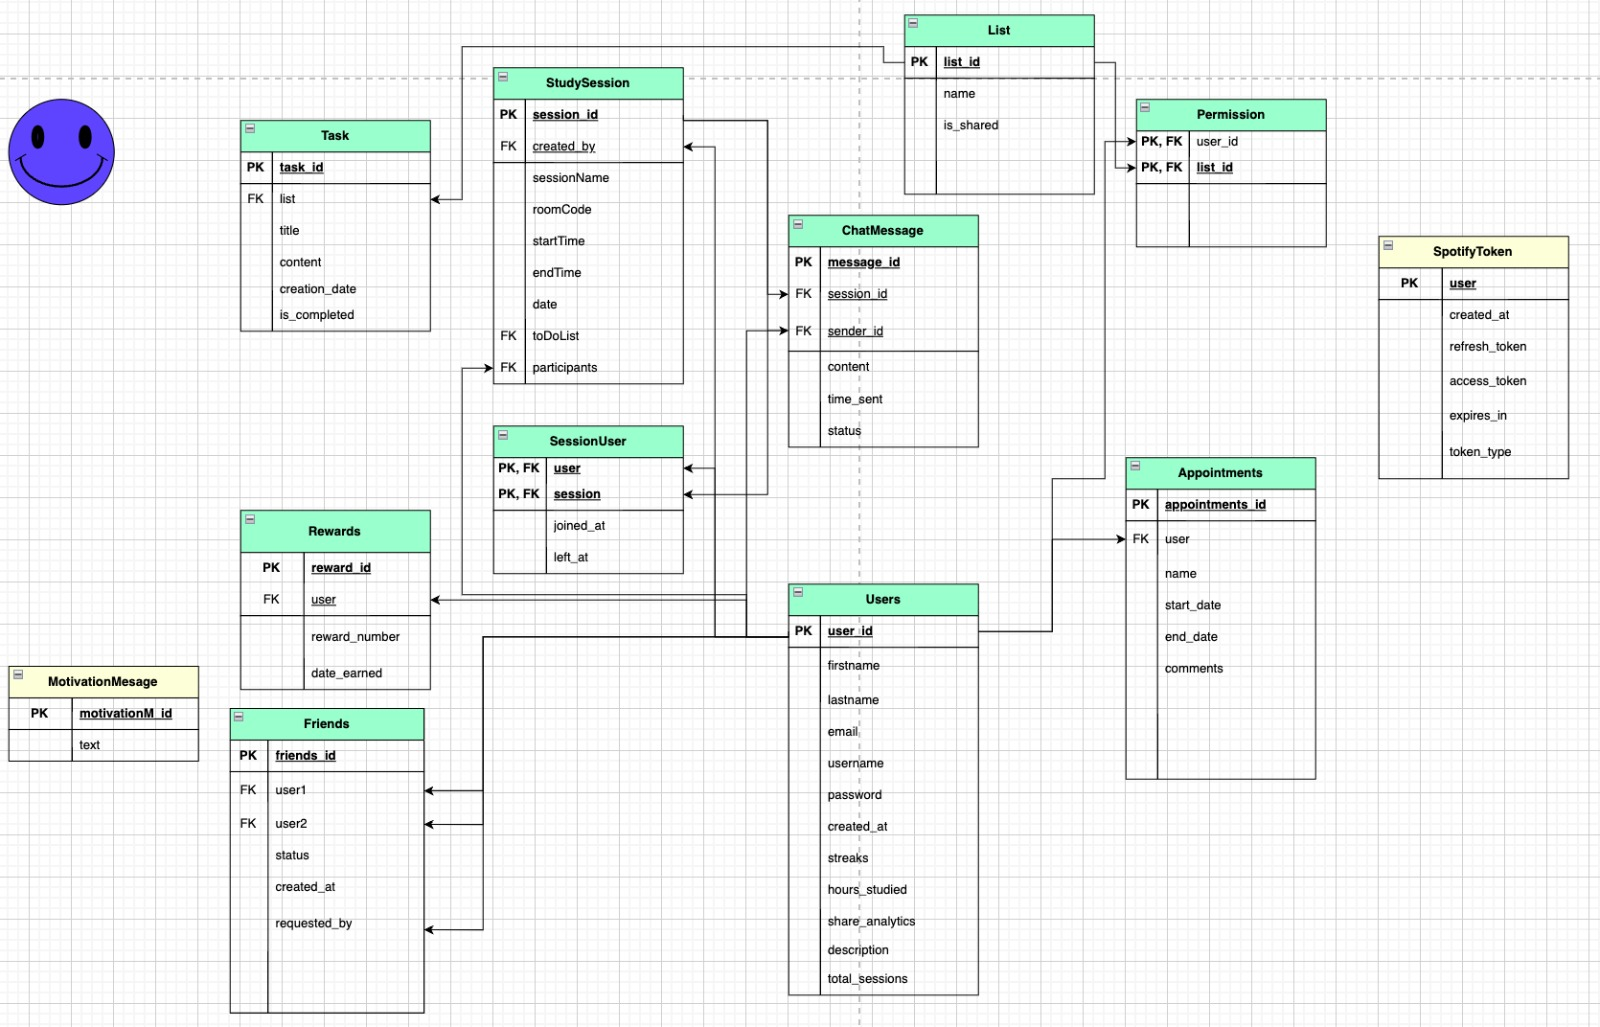
\includegraphics[width=1\linewidth]{ER-diagram}
    \caption{Finalised ER Diagram}
    \label{fig:er-diagram}
\end{figure}


\section{Implementation Details}
\label{sect:implementation-details}
\subsection{Initial Design Plan}
We gained inspiration from existing study group pages and the elements / components needed by the students. We brainstormed and mapped components onto paper: added components block-wise like a grid on the dashboard and group study pages. We used Figma to start designing how the UI components placement, colour scheme and overall presentation/layout of all the different pages: \textit{Login, Welcome Page, Dashboard, Group Study Room.}

\subsection{Finalised Features} Through the elimination process, we nailed down the ideas that reflected the goals of our project and made our idea unique. 
\begin{itemize}
    \item \textbf{To-Do List (shared):} This allows the user to create individual lists for themselves and separate group lists (when working as a group). 
    \item \textbf{Shared Materials:} Allows multiple users, in a group study session, to be able to share materials with each other in, but this is only active whilst the session is alive.
    \item \textbf{Timer:}This feature allows the user to schedule breaks within their desired focus time.
    \item \textbf{Chat box:} allowing users to communicate, while present in the group study room. This allows the user to be less distracted then on audio/video call, ensuring that communication is catered towards finishing the tasks.
    \item \textbf{Motivational Message:} These are randomly generated inspirational quotes, to encourage the user to continue studying and stay focused.
    \item \textbf{Profile Box:}  User can change their avatar (based on uploaded pictures from their device) and write a user description. This gives the user more creativity to customise their avatar and description to match them.
    \item \textbf{Statistics :} Collects data on the number of consecutive days they joined a study session (streaks) and also calculates the average time spent in the study room. This allows the user to track their time and remember to stay consistent with their studies. The user also has the option to share their data with friends, for some healthy competition. 
    \item \textbf{Friends List:} This allows the user to see the: friends list (which users they have accepted as friends), pending requests from new users, accepted friend requests and search for different friends. 
    \item \textbf{Calender:} This allows the user to schedule events, classes, exams and other assignment deadlines to keep up with and clearly organise a busy schedule.
    \item \textbf{Badges:} This is a type of reward system, that encourages the student to complete certain goals in order to achieve them. For instance, completing a certain number of hours, number of tasks etc.
    \item \textbf{Music: }Background music helps in productivity and makes the user feel more at ease when studying. It also helps avoid distraction and boosts motivation, each user independently listens to a track of their choice. Using Spotify API, premium users can control playback, helping to limit phone distraction.
    \item \textbf{Joined Users:} This allows the participants who are already in the room, to see who has joined.
    \item \textbf{Create/Join Room:} This allows user to create a study room/join a study room. This is the foundation of the project, which creates a platform for users to share learning materials, to-do list tasks, chat with each other, independently control timer and  music features.  And be inspired by the motivational messages. 

\end{itemize}

The \textbf{Welcome Page/Login/Sign Up} is simply designed to entice the user to login/sign up, using a vibrant pattern/colour scheme, is simplicity provides robust functionality to get the user seamlessly enter the platform.

\subsection{Dashboard and Group Study Page}
In both the \textbf{Dashboard} and \textbf{Group Study Page}, the components are arranged in columns. 

\begin{itemize}
    \item The \textbf{Dashboard} consists of: Profile Box, To-Do List, Join/Create Study Room, Friend Requests, Calendar, and Badges.
    \item The \textbf{Group Study Page} consists of: To-Do List, Shared Materials, Music, Joined Users, Motivational Message, Timer, and Chat Box.
\end{itemize}
 
This page has been tailored to the expectation of collaborative studies, where we have included the ability to exchange study materials with all users in the group, participate in educational conversations and create shared to do lists to complete with your team. 

There also additional features to help avoid distraction and boost maximum productivity with Timers, Music, Motivational quotes. 
The Group Study page includes a taskbar, to provide further functionalities to leave the group study room, copy-paste the room code, music feature and present the room code.

All these design decisions are reflected in the final product, the orientation of all these components has also been carefully crafted to meet the user's needs and expectations. Moreover, the layout has been slightly altered overtime to enhance user experience.



\section{Alternative Considerations}
\label{sect:alternative-considerations}
We researched and discussed several possibilities for different aspects of the project, from our tech stack to which features we should implement.

\subsection{Features}
Initially, we had planned to use an ChatGPT API to create small quizzes using the documents uploaded to the shared materials box in the group study room; however, we had to de-prioritise this feature due to lack of time, as well as us considering the other features to be of greater importance.

We also considered allowing users to join their friends' study rooms without a room code, i.e. implement a feature that lets you see which of your friends are currently online or in a study room, and being able to join them in that study room without needing to enter the room code. After much deliberation, we decided to put this feature on the back burner since users may not want their friends to be able to suddenly enter into a study room without their permission, particularly considering that most students have different study groups for different purposes and may not want members of one group mixing with another.


\subsection{Tech Stack}
We had decided on using Django for the backend of the project and React for the frontend quite early on in the timeline, however, it took us a while to settle on which database to use in order to store user data. In particular, we could not choose between SQLite and Firebase. 

Half of us wanted to stick to what we knew by using SQLite since that is what we used in the Small Group Project, whereas the other half wanted to learn something new and extend ourselves. In the end, we decided to use both; \begin{itemize}
    \item \textbf{Django Models} for structured data.
    \item \textbf{Firebase} for multimedia storage.
\end{itemize}

Our chosen architecture follows a modular and scalable approach, ensuring separation of concerns between the frontend, backend, and database. The React frontend provides a dynamic user experience and the Django backend was selected for its robustness in handling authentication, session management, and complex data processing. By using Firebase for multimedia storage, we had an option to provide real-time file sharing, which we would not have done with just the use of Django models. This architecture follows software engineering best practices such as scalability, maintainability, and modularity, ensuring that features can be expanded in future iterations without major restructuring.


\subsection{Deployment}
To ensure a swift and clean deployment, we planned and moved ahead with PythonAnywhere to deploy the backend (Django). Though this proved to be an oversight on our part as the free version of PythonAnywhere did not support websockets, which we had used in multiple features of the group study room - such as the chat and shared to-do list. After some further research and inquiring with other groups with a similar tech stack, we came to know about Render, which is what we finally used to deploy the backend.

Although we were unanimous in our decision for the backend deployment, the frontend deployment tools took slightly more time and effort. We looked into Azure, Cloudflare, Heroku, and a few other services, however they all did not have a free plan that met our needs. In the end, we came across Vercel and it seemed to meet all our requirements. It was very convenient to use Vercel since it is linked to our GitHub repository meaning it redeployed every time main is updated which means we do not have to dedicate extra time to deploying the frontend regularly.

\section{Changes During Development}
\label{sect:changes-during-development}

\subsection{Changes in UI Design}
The base design of the original UI utilised a limited range of colours and was slightly more flat in appearance, in addition to the repeated use of the black sans serif font. Our advisor suggested that we should ensure the UI was more cohesive, and that the study room component should be placed in the centre of the dashboard as it was our website’s unique selling point, as opposed to the profile component; consequently, we implemented this advice, and our profile box component was placed to the left. 
One of Onessa’s tasks was to ensure the UI flowed more and cultivated a more dynamic, inviting feel to the website. For the welcome page, her aim was to create a “mango” aesthetic true to the mango cat logo/ mascot of the website, utilising a range of reds and oranges for the upper and lower borders, with  mango emojis in the corner of the welcome box! This choice of bold and bright colours for the first page the users would see, intends to evoke a burst of energy and elation towards the notion of studying, which is universally seen as a boring task. 

The login and sign-up pages had more of a “peach” aesthetic with a range of pinks, yellows and light oranges. This would then transition into the “lighter” pink and blue aesthetic used for the dashboard, maintaining the same subtle and light colour theme throughout that was originally intended for the UI. Then it seamlessly morphs into the benevolent, rich deep purple and soft purple-blue colour schemes on the group study room page, to allow the room to feel immersive and inviting while also elevating user concentration. On this page the music, customisation, exit and copy code buttons were placed on the border as opposed to in the middle of the group study page where you can see the users in the room which was the case earlier, with the icons being buttons themselves as opposed to being on rounded buttons, as they are auxiliary to the room’s key components, and to ensure the central study area was less cluttered. 

The “Orbitron” font, with a subtle greyish shadow, was a unique choice that she used for the titles of each page in the borders; its geometric, futuristic style intends to motivate students to aim for the brightest future that they dream of having, which correlates with wanting to study/ focus more to achieve this. As for the other text on the pages, she kept the inter sans serif fonts but capitalised them and added subtle playful, pinkish shadows, accentuating the dynamic and cosy overall effect of the website. 

Finally, there was a smiley face slider that was originally going to be on the group study page but it was relocated to the analytics container on the dashboard, allowing the user to choose whether their friends could see their study statistics. This was an effective design choice; it ensured the dashboard was more streamlined while also enabling users to have more control over their privacy. 

\subsection{Changes in Implementation}
\textbf{Deployment Challenges} 

Upon first deployment to PythonAnywhere, a limitation we faced was that there was a paid tier for supporting Websockets, which a plethora of the key real-time features of our website relied upon. Thus, we mitigated by relocating the app to Vercel and Render, which possessed more scalable methods of hosting and real-time functionality, enabling us to achieve this for free. This uninterrupted, free inclusion of WebSockets fulfilled the technical and financial limitations of the project.

\textbf{Adapting Music Feature Integration for Accessibility}

The Spotify API used for the music component of the group study room possessed a large limitation, which we were initially unaware of. The reliance on Spotify Premium caused accessibility problems for users without this subscription. Hence after pondering over this as a team, we transitioned to integrating free music sources, giving us a nice availability of audio content; we were able to include a range of tracks that members of our group enjoyed, and as students ourselves, believed created the perfect ambience for studying as a group, from 2010 summer themed tracks to Pokemon and Animal Crossing tracks, adored by a range of students. From a user's standpoint, initially sticking to just the Spotify Premium API could be viewed as less inclusive and may dissuade them from wanting to use the group study room if they frequently listen to music while studying and dislike ads.

\textbf{User Authentication Workflow Refinements}

User authentication at first had issues with various accounts logged into the same browser using multiple tabs, resulting in token collision and unauthorised overridings, so only the most recently logged in user would be logged in on all tabs. We solved this by enforcing one active session per browser. However, lingering authentication cookies would sometimes prevent the user from logging in after partial sign-outs (for e.g, if the user lost connection, causing them to unintentionally log out). This was solved by implementing an automatic logout feature of all the user's logged in accounts triggered by them refreshing the page, enabling more consistent session management for the user.

\textbf{Evolution of the Calendar Feature}

The calendar feature, which started off as a feature that has a smaller preview on the dashboard and a large view when clicked on, evolved considerably during development. We replaced this preview with a streamlined calendar emoji button, reclaiming space on the interface for higher priority components. It also previously required manually changing the status of an event on the calendar to facilitate event colour coding, however that was optimised to be automatic given when the events took place: events in the past, present and future were represented with different colours respectively. The feature's expansion points to how it has grown into a central tool for time management within the application, allowing users to visually prioritise tasks with more ease.

\section{Justification of Architectural Choices}
\label{sect:justification}
Our architecture follows software engineering best practices:
\begin{itemize}
    \item \textbf{Modularity:} Frontend (React), backend (Django), and database (Firebase/Django Models) are separated.
    \item \textbf{Scalability:} Features can be expanded without major restructuring.
    \item \textbf{Efficiency:} React ensures fast rendering, Django manages authentication, and Firebase handles real-time storage.
\end{itemize}